\section{Arithmetic Programs}
Suppose we have some algebra \(\mathbb{A}\): we can represent and deal with finite sequences of 
operations, called \emph{expressions}, between elements of \(\mathbb{A}\) and/or variables over 
\(\mathbb{A}\).

For example, given the expression \(x^2 + x + 1\) over \(\mathbb{R}\left[x\right]\), we might be 
interested to know what is the \emph{evaluation} of the expression given some value for \(x\).

\begin{definition}[Arithmetic formula]
  Given an algebraic structure \(\mathbb{A} = \Tuple{A, \odot_1, \dots, \odot_n}\), an explicit 
  arithmetic formula over \(\mathbb{A}\) is any expression \(\varphi \) of the kind:
  \begin{align*}
    & \varphi \equiv a && \forall a \in A \\ 
    & \varphi \equiv x && \textnormal{with \(x\) variable over \(A\)} \\
    & \varphi \equiv \varphi_1 \odot_i \varphi_2 && 
    \forall i \le n, \varphi_1 \neq \varphi, \varphi_2 \neq \varphi
  \end{align*}
  Additionally, an implicit (or succint) arithmetic formula also allows expressions of the kind:
  \begin{align*}
    & \varphi \equiv \call{\odot_i^k}{\varphi_1} && 
    \forall i \le n, \forall k \in \mathbb{N}, \varphi_1 \neq \varphi
  \end{align*}
\end{definition}

\begin{remark}
  It is always possible to translate an implicit formula into an equivalent explicit one.
  We denote the explicit version of an implciit formula \(\varphi \) with \(\explicit{\varphi}\).
  For some particular structures, such as fields, this translation can be specialized. 
\end{remark}

Usually, we deal with arithmetic formulae over some field (or ring) \(\mathbb{F}\), in which case 
implicit arithmetic expressions are equivalent to multi-variate polynomials.
\begin{example}\label{ex:arithmetic_formula}
  Consider the field \(\mathbb{Z}_{13} = \Tuple{\Set{0, \dots, 12}, \oplus_{13}, \otimes_{13}}\).
  For ease of notation, \(\oplus_{13}\) is equivalent to \(+\) and \(\otimes_{13}\) is equivalent 
  to juxtaposition. 
  A valid implicit arithemtic formula over \(\mathbb{Z}_{13}\) then would be:
  \[\varphi = x_{2}\Parens*{x_{1}^{3} + 4x_{2} + 5}\]
  Since in a finite field we can see multiplication by a constant as repeated addition, i.e. 
  \(c \otimes x = \call{\oplus^{c}}{x}\), the explicit version of \(\varphi \) then is:
  \[\explicit{\varphi} = x_{2}\Parens*{x_{1}x_{1}x_{1} + x_{2} + x_{2} + x_{2} + x_{2} + 5}\]
\end{example} 

It is possible to visually represent an arithmetic formula using a particualr kind of labeled 
\emph{directed acyclic graph} (DAG).
\begin{definition}[Arithmetic circuit]
  An arithmetic circuit over an algebra \(\mathbb{A} = \Tuple{A, \odot_1, \dots, \odot_n}\) and a 
  set of variables \(X\) over \(\mathbb{A}\) is a triple \(\mathcal{G} = \Tuple{V, E, L}\) where 
  \(V\) is the set of vertices, \(E \subseteq V \times V\) is the set of edges, and 
  \(L\colon V \to A \cup X \cup \Parens*{\Set{\odot_1, \dots, \odot_n} \times \mathbb{N}}\) is 
  the vertex labeling map, such that, \(\forall v \in V\):
  \begin{align*}
    & \call{L}{v} \in A && \implies \nexists w \in V\colon \Tuple{w, v} \in E
    && \textnormal{(no in-edges for constant nodes)} \\
    & \call{L}{v} \in X && \implies \nexists w \in V\colon \Tuple{w, v} \in E
    && \textnormal{(no in-edges for variable nodes)} \\
    & \forall i \le n\colon \odot_i \in \call{L}{v} && \implies \abs{\Set{\Tuple{w, v}}_{w \in V} \cap E} = \abs{\odot_i}
    && \textnormal{(exactly \(\abs{\odot_i}\) in-edges for \(\odot_i\) nodes)}
  \end{align*}
\end{definition}

Given any explicit arithmetic formula \(\varphi \) over an algebra \(\mathbb{A}\) and a set of 
variables \(X\), we can build the corresponding arithmetic circuit \(\mathcal{G} = \Tuple{V, E, L}\) 
and partition \(V\) in the following way: 
\begin{itemize}
  \item \emph{Constant vertices}: denoted 
    \(\mathcal{G}_{const} = \Set{v \mid v \in V \wedge \call{L}{v} \in \mathbb{A}}\) 
  \item \emph{Variable vertices}: denoted 
    \(\mathcal{G}_{var} = \Set{v \mid v \in V \wedge \call{L}{v} \in X}\).
  \item \emph{Operation vertices}: denoted 
    \(\mathcal{G}_{\odot_i} = \Set{v \mid v \in V \wedge \odot_i \in \call{L}{v}}\).
  \item \emph{Input vertices}, denoted 
    \(\mathcal{G}_{in} = \mathcal{G}_{const} \cup \mathcal{G}_{var}\).
  \item \emph{Output vertices}, denoted 
    \(\mathcal{G}_{out} = \Set{v \mid v \in V \wedge \nexists w\colon \Tuple{v, w} \in E}\).
  \item \emph{Input/Output vertices}, denoted \(\mathcal{G}_{IO} = \mathcal{G}_{in} \cup \mathcal{G}_{out}\).
\end{itemize}

\begin{example}
  \Cref{fig:arithmetic_circuit} shows the arithmetic circuit derived from the formula shown in 
  \Cref{ex:arithmetic_formula}.
  We can see the two variable vertices \(x_1\) and \(x_2\) which are also input vertices, the 
  constant vertex \(5\), which is an input vertex too, the
  addition vertices \(\oplus_1, \dots, \oplus_5\) and the multiplication vertices 
  \(\otimes_1, \otimes_2, \otimes_3\), of which the latter is also an output vertex.
\end{example}

\begin{figure}
	\centering
	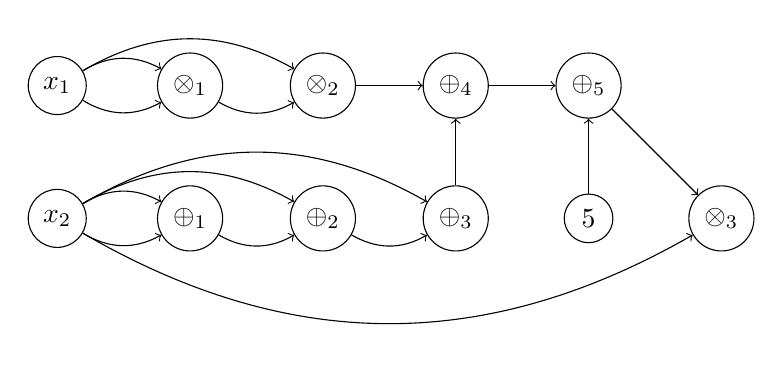
\begin{tikzpicture}[node distance={48pt}, node/.style = {draw, circle}]
		\node[node] (x1) {\(x_1\)};
		\node[node] (x2) [below of=x1] {\(x_2\)};
		\node[node] (m1) [right of=x1] {\(\otimes_1\)};
		\node[node] (m2) [right of=m1] {\(\otimes_2\)};
		\node[node] (a1) [right of=x2] {\(\oplus_1\)};
		\node[node] (a2) [right of=a1] {\(\oplus_2\)};
		\node[node] (a3) [right of=a2] {\(\oplus_3\)};
		\node[node] (a4) [right of=m2] {\(\oplus_4\)};
		\node[node] (a5) [right of=a4] {\(\oplus_5\)};
		\node[node] (5) [below of=a5] {\(5\)};
		\node[node] (m3) [right of=5] {\(\otimes_3\)};
		\draw[->] (x1) to [bend left] (m1);
		\draw[->] (x1) to [bend right] (m1);
		\draw[->] (x1) to [bend left] (m2);
		\draw[->] (m1) to [bend right] (m2);
		\draw[->] (x2) to [bend left] (a1);
		\draw[->] (x2) to [bend left] (a2);
		\draw[->] (x2) to [bend left] (a3);
		\draw[->] (x2) to [bend right] (a1);
		\draw[->] (a1) to [bend right] (a2);
		\draw[->] (a2) to [bend right] (a3);
		\draw[->] (m2) to (a4);
		\draw[->] (a3) to (a4);
		\draw[->] (a4) to (a5);
		\draw[->] (5) to (a5);
		\draw[->] (a5) to (m3);
		\draw[->] (x2) to [bend right] (m3);

	\end{tikzpicture}
	\caption{Arithmetic circuit of the formula shown in \Cref{ex:arithmetic_formula}.}\label{fig:arithmetic_circuit}
\end{figure}

Since arithmetic circuits contain no cycles, they can only be used to represent a fixed number 
of operations (aka \emph{bounded computations}).
